%
\documentclass[12pt]{article}

\usepackage{fullpage}
\usepackage{setspace}
\usepackage{endnotes}
\usepackage{amsmath}
\usepackage{amsfonts}
\usepackage{amssymb}
\usepackage{mathrsfs}
\usepackage{calrsfs}
\usepackage{rotating}
\usepackage{dcolumn}
\usepackage{longtable}
\usepackage{microtype}
\usepackage{graphicx}
\usepackage{url}
\usepackage{natbib}
\bibpunct{(}{)}{;}{a}{}{,}
\usepackage{framed}
\usepackage{lipsum}
\usepackage[font=small,labelfont=sc]{caption}
 \usepackage{float}
\restylefloat{table}
\usepackage[usenames,dvipsnames]{color}

% refs and pdf meta
\usepackage{hyperref}
\hypersetup{
 pdftitle={Reasonable Measures of Uncertainty Under Separation}, % title
 pdfauthor={Carlisle Rainey}, % author
 pdfkeywords={logistic regression}{separation}{Firth}{Cauchy}{MCMC}
 pdfnewwindow=true, % links in new window
 colorlinks=true, % false: boxed links; true: colored links
 linkcolor=BrickRed, % color of internal links
 citecolor=BrickRed, % color of links to bibliography
 filecolor=BrickRed, % color of file links
 urlcolor=BrickRed % color of external links
}

% Set up theorems, etc.
\usepackage{amsthm}
\newtheorem{lemma}{Lemma}
\newtheorem{proposition}{Proposition}
\newtheorem{theorem}{Theorem}
\newtheorem{claim}{Claim}
\newtheorem{assumption}{Assumption}
\newtheorem{defn}{Definition}


% Allow restating theorems (for the Appendix)
\usepackage{thmtools}
\usepackage{thm-restate}
\usepackage{cleveref}

% Set up fonts the way I like
\usepackage{tgpagella}
\usepackage[T1]{fontenc}
%\usepackage[T1]{fontenc}
\usepackage[bitstream-charter]{mathdesign}


%Redefine the first level
\renewcommand{\theenumi}{\arabic{enumi}.}
\renewcommand{\labelenumi}{\theenumi}
%Redefine the second level
\renewcommand{\theenumii}{\alph{enumii}.}
\renewcommand{\labelenumii}{\theenumii}
%Redefine the third level
\renewcommand{\theenumiii}{\roman{enumiii}.}
\renewcommand{\labelenumiii}{\theenumiii}
%Redefine the fourth level
\renewcommand{\theenumiv}{\Alph{enumiv}.}
\renewcommand{\labelenumiv}{\theenumiv}


\parskip=0pt
\parindent=20pt
\usepackage{lscape}
\singlespace

% Create footnote command so that my name
% has an asterisk rather than a one.
\long\def\symbolfootnote[#1]#2{\begingroup%
\def\thefootnote{\fnsymbol{footnote}}\footnote[#1]{#2}\endgroup}

\begin{document}


\begin{center}
{\LARGE Dealing with Separation in Logistic Regression Models\symbolfootnote[1]{I thank Charles Barrilleaux for presenting me with the methodological issues that this paper addresses and Kelly McCaskey for excellent research assistance. Thanks to Mark Bell and Nicholas Miller for making their data available to me. The analyses presented here were conducted with \texttt{R} 3.1.0. All data and computer code necessary for replication are available at \href{https://github.com/carlislerainey/priors.for-separation}{github.com/carlislerainey/priors-for-separation}.}}

\vspace{10mm}

Carlisle Rainey\symbolfootnote[2]{Carlisle Rainey is Assistant Professor of Political Science, University at Buffalo, SUNY, 520 Park Hall, Buffalo, NY 14260 (\href{mailto:rcrainey@buffalo.edu}{rcrainey@buffalo.edu}).}

\end{center}

% remove page number from first page
\thispagestyle{empty}

% abstract
\vspace{10mm}
{\centerline{\textsc{Abstract}}}
\begin{quote}\noindent When facing data sets with small numbers of observations or ``rare events,'' political scientists often encounter important explanatory variables that perfectly predict binary events or non-events. In this situation, maximum likelihood provides implausible estimates and the researcher must incorporate some form of prior information into the model. The most sophisticated research uses Jeffreys' invariant prior to stabilize the estimates. Jeffreys' prior has the advantage of being automatic, but I show that, in many cases, it offers too much prior information, producing confidence intervals that are much too narrow. The choice of a more reasonable prior can lead to different substantive conclusions about the likely magnitude of an effect. I offer practical advice for and substantive examples of choosing an informative prior distribution, estimating the subsequent model, and summarizing the results.\end{quote}


\newpage
\doublespace

Separation, in which an explanatory variable perfectly predicts some observations, remains a problem in political science research (e.g., Reiter 2014; Barrilleaux and Rainey 2014; Leeman and Mares 2014; and Bell and Miller 2014). Zorn (2005) offers the most principled solution to the problem of separation by suggesting that researchers maximizes a penalized version of the usual likelihood approach. However, when implementing Zorn?s suggested approach, substantive researchers face at least two problems. First, the penalty suggested by Zorn is designed for bias reduction in logistic regression models and not for handling separation. Whether the suggested penalty approximates actual prior information in particular substantive settings remains an open and problem-specific question. Second, interpreting logistic regression coefficients requires focusing a substantively meaningful quantities of interest (e.g., first-difference, risk-ratio). However, Zorn (2005) notes that the usual normal approximation suggested by King, Tomz, and Wittenberg is not suitable under separation. Thus, researchers have no way to obtain accurate confidence intervals around their quantities of interest.

In this paper, I introduce the conceptual and computational tools to solve these two problems. I make four specific contributions. First, I use statistical theory and two applied examples to demonstrate the important of choosing a prior distribution that represents actual prior information and conducting robustness checks using a variety of prior distributions. Second, I introduce the concept of a partial prior predictive distribution, a powerful tool in understanding the information provided by the prior when facing separation, as well as the software necessary to compute the partial prior predictive distribution. Thirdly, I introduce a set of useful tools for simulating from the posterior distribution without relying on a normal approximation and graphically and numerically summarizing the inferences.

\section*{The Logistic Regression Model}

Political scientists commonly use logistic regression to model the probability of events such as war (e.g., \citealt{Fearon1994}), policy adoption (e.g., \citealt{BerryBerry1990}), turning out to vote (e.g., \citealt{WolfingerRosenstone1980}), and government formation (e.g., \citealt{MartinStevenson2001}). In the typical situation, the researcher uses an $n \times (k + 1)$ design matrix $X$ consisting of an intercept and $k$ explanatory variables to model a vector of $n$ binary outcomes $y$, where $y_i \in \{0, 1\}$, using the model $\text{Pr}(y_i) = \text{Pr}(y_i = 1~|~ X_i) = \dfrac{1}{1 + e^{-X_i\beta}}$, where $\beta$ is a parameter vector of length $k + 1$. Using this model, it is straightforward to calculate the likelihood function 

\begin{equation}\nonumber
\text{Pr}(y | \beta) = L(\beta | y) = \displaystyle \prod_{i = 1}^n \left[\left( \dfrac{1}{1 + e^{-X_i\beta}}\right)^{y_i} + \left( \dfrac{1}{1 + e^{-X_i\beta}}\right)^{1 - y_i}\right]\text{.}
\end{equation}

%\noindent As usual, one can take the natural logarithm of both sides to calculate the log-likelihood function 
%
%\begin{equation}\nonumber
%\log L(\beta | y) = \displaystyle \sum_{i = 1}^n \left[y_i \log \left( \dfrac{1}{1 + e^{-X_i\beta}}\right) + (1 - y_i) \log \left( \dfrac{1}{1 + e^{-X_i\beta}}\right)\right]
%\end{equation}
%
%\noindent and take the derivatives of the log-likelihood function to obtain the score function
%
%\begin{equation}\nonumber
%\dfrac{\partial \log L(\beta | y)}{\partial \beta} = \displaystyle \sum_{i = 1}^n\left(y_i - \dfrac{1}{1 + e^{-X_i\beta}}\right)X_i\text{.}
%\end{equation}

Researchers routinely obtain maximum likelihood estimates $\hat{\beta}^{mle}$ of the model parameters $\beta$ by find the vector $\beta$ that maximizes $L$ (i.e., maximizing the likelihood of the observed data). While this approach works quite well in most applications, it fails in a situation known as separation \citep{Zorn2005}.

\section*{Separation}

Separation occurs in models of binary outcome data when one explanatory variable perfectly predicts zeros, ones, or both.\footnote{Separation can also occur when a \emph{combination} of explanatory variables perfectly predicts zeros, ones, or both, see \cite{LesaffreAlbert1989}.} \textit{Complete separation} occurs when the ``problematic'' explanatory variable $s_i$ (for \underline{s}eparating explanatory variable) perfectly predicts both zeros \emph{and} ones. \textit{Quasicomplete separation} occurs when $s_i$ perfectly predicts either zeros \emph{or} ones, but not both (\citealt{AlbertAnderson1984}, \citealt{Zorn2005}). \textit{Overlap}, the ideal case, occurs when there is no such $s_i$. When the data overlap, the usual maximum likelihood estimates exist and provide reasonable estimates of parameters. However, under complete or quasicomplete separation, finite maximum likelihood estimates do not exist and the usual method of calculating standard errors fails (\citealt{AlbertAnderson1984, Zorn2005}).

Complete separation occurs when $s_i$ perfectly predicts \emph{both} zeros \emph{and} ones. For example, suppose a dichotomous explanatory variable $s_i$ , such that $y_i = 0$ for $s_i = 0$ and $y_i = 1$ for $s_i = 1$. To maximize the likelihood of the observed data, the ``S''-shaped logistic regression curve must assign $\text{Pr}(y_i) = \frac{1}{1 + e^{-X_i\beta}} = 0$ when $s_i  = 0$ and $\text{Pr}(y_i) = \frac{1}{1 + e^{-X_i\beta}} = 1$ when $s_i = 1$. Since the logistic regression curve lies strictly between zero and one, this likelihood cannot be achieved, only approached asymptotically as the coefficient $\beta_s$ for $s_i$ approaches infinity. Thus, the likelihood function under complete separation is monotonic, which implies that a finite maximum likelihood estimate does not exist.\footnote{Although coefficient estimates under separation are infinite \emph{in theory}, the hill-climbing algorithms approximate the infinite estimates with large, finite values \emph{in practice}. These approximations increase with the precision of the algorithm. See \cite{Zorn2005} for an illustration using software in Stata and R.}

Quasicomplete separation occurs when $s_i$ perfectly predicts \emph{either} zeros \emph{or} ones. For example, suppose that,  when $s_i = 0$, sometimes $y_i = 1$ and other times $y_i = 0$, but $y_i = 1$ \emph{always} equals zero when $s_i = 1$. This situation occurs often in applied political science research with binary inputs. To maximize the likelihood of the observed data, the ``S''-shaped logistic regression curve must assign $\text{Pr}(y_i) = \frac{1}{1 + e^{-X_i\beta}} \in (0, 1)$ when $s_i  = 0$ and $\text{Pr}(y_i) = \frac{1}{1 + e^{-X_i\beta}} = 1$ when $s_i = 1$. Again, since the logistic regression curve lies strictly between zero and one, this likelihood cannot be achieved, only approached asymptotically. Thus, the likelihood function under quasicomplete separation is also monotonic, which again implies that the maximum likelihood estimate does not exist.

For example, \cite{BarrilleauxRainey2014} find that no Democratic governors opposed the medicaid expansion under the Affordable Care Act, leading to a maximum likelihood estimate of positive infinity for the coefficient for the indicator of Republican governors. Similarly, \cite{Rauchhaus2009} (see \citealt{BellMiller2014}) finds no instances of states with nuclear weapons engaging in war with each other, leading to an estimated coefficient of negative infinity for the variable indicating symmetric nuclear dyads (in which both states possess nuclear weapons). To maximize the likelihood in this situations, the model must assign probabilities of zero to states with Democratic governors and probabilities of zero to symmetric nuclear dyads. Because the logistic regression curve lies strictly above zero, this cannot happen, though it can be approached asymptotically as the coefficient for $s_i$ goes to negative infinity. 

For simplicity, this paper focuses the more common situation of quasicomplete separation. However, the ideas apply equally well to the less common situation of complete separation.  For convenience, I say that the ``direction of the separation'' is positive if and only if $s_i = 1 \implies y_i = 1$ \underline{or} $s_i = 0 \implies y_i = 0$ and that the direction of separation is negative if and only if $s_i = 0 \implies y_i = 1$ \underline{or} $s_i = 1 \implies y_i = 0$. Thus, $\hat{\beta}^{mle} = +\infty$ when the direction of the estimate is positive, and $\hat{\beta}^{mle} = -\infty$ when the direction of the estimate is negative.

%\begin{figure}[H]
%\begin{center}
%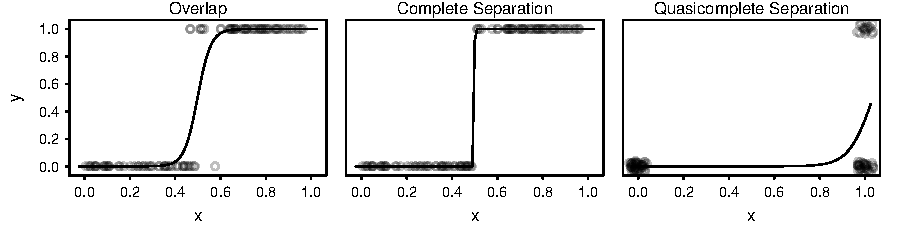
\includegraphics[scale = 1]{figs/illustrate-separation.pdf}
%%\vspace{-10mm}
%\end{center}
%\caption{This figure illustrates overlap, complete separation, and quasicomplete separation as defined by \cite{AlbertAnderson1984}. The maximum likelihood estimates only exist under overlap. Under complete and quasicomplete separation, maximum likelihood fails, returning infinite estimates and standard errors.}\label{fig:illustrating_separation}
%\end{figure}

%\begin{table}[H]
%\begin{center}
%\begin{footnotesize}
%\begin{tabular}{l c c | c c | c c }
%\hline
% & \multicolumn{2}{c}{Overlap}&\multicolumn{2}{c}{Complete Separation}&\multicolumn{2}{c}{Quasicomplete Separation}\\
%               & $\epsilon = 10^{-8}$ & $\epsilon = 10^{-16}$ & $\epsilon = 10^{-8}$ & $\epsilon = 10^{-16}$ & $\epsilon = 10^{-8}$ & $\epsilon = 10^{-16}$ \\
%\hline
%constant    & $-17.05$ & $-17.05$ & $-739.27$     & $-739.27$     & $-19.57$    & $-26.57$     \\
%               & $(5.79)$      & $(5.79)$      & $(139744.58)$ & $(139744.58)$ & $(1520.85)$ & $(50363.70)$ \\
%x              & $34.19$  & $34.19$  & $1483.21$     & $1483.21$     & $18.90$     & $25.90$      \\
%               & $(11.92)$     & $(11.92)$     & $(280801.40)$ & $(280801.40)$ & $(1520.85)$ & $(50363.70)$ \\
%\hline
%Log Likelihood & -9.74         & -9.74         & 0.00          & 0.00          & -32.05      & -32.05       \\
%Num. obs.      & 100           & 100           & 100           & 100           & 100         & 100          \\
%\hline
%\multicolumn{7}{l}{Standard errors in parentheses.}
%\end{tabular}
%\caption{A table providing estimates based on the data shown in Figure \ref{fig:illustrating_separation} using the R function \texttt{glm()} varying the convergence tolerance under overlap, complete separation, and quasicomplete separation. Notice that the estimation algorithm returns estimates and standard errors arbitrarily close to infinity under both types of separation as the tolerances shrinks to zero.}
%\label{tab:illustrating_separation}
%\end{footnotesize}
%\end{center}
%\end{table}
%
%Perhaps more starkly, notice  that the strong pattern in the middle panel of Figure \ref{fig:illustrating_separation} does not produce statistically significant result. This is because the likelihood is essentially flat around the ``maximum'' found by the hill-climbing algorithm. As the region around the maximum flattens, the estimates of the standard errors increases. Thus, separation leads to implausible large estimates \textit{and} standard errors. Notice, for example, that while the data in the middle and right panel would almost never occur under the null hypothesis of no relationship, none of the estimates are statistically significant.

\section*{Solutions to Separation}

The maximum likelihood (ML) framework requires the researcher to find the parameter vector that ``maximizes the likelihood of the observed data.'' Of course, infinite coefficients \textit{always} generate separated data, while finite coefficients only \emph{sometimes} generate separation. Thus, under separation, the ML can only produce infinite estimates.

Before addressing potential solutions to this problem, let me mention two unsatisfactory ``solutions'' found in applied work. In some cases, researchers simply ignore the problem of separation and interpret the large estimates and standard errors as though these are reasonable. However, this approach leads researchers to overstate the magnitude of the effect and the uncertainty of the estimates. Secondly, researches sometimes ``solve'' the problem of separation by dropping the separating variable from the model. \citet[pp. 161-162]{Zorn2005} correctly dismisses this approach:

\begin{quote}
As a practical matter, separation forces the analyst to choose from a number of problematic alternatives for dealing with the problem. The most widely used ``solution'' is simply to omit the offending variable or variables from the analysis. In political science, this is the approach taken in a number of studies in international relations, comparative politics, and American politics. It is also the dominant approach in sociology, economics, and the other social sciences, and it is the recommended method in a few prominent texts in statistics and econometrics. Of course, this alternative is a particularly unattractive one; omitting a covariate that clearly bears a strong relationship to the phenomenon of interest is nothing more than deliberate specification bias.
\end{quote}

One principled solution is to build prior information $p(\beta)$ (the same prior information that leads researchers to deem infinite coefficients ``implausibly large'') into the model using Bayes' rule, so that 

\begin{equation}\nonumber
p(\beta|y) = \dfrac{\overbrace{p(y|\beta)}^{\text{likelihood}}\overbrace{p(\beta)}^{\text{prior}}}{\int p(y|\beta)p(\beta) d\beta}~\text{.}
\end{equation}

\noindent In this case, the estimate switches to from the maximum likelihood estimate to a summary of the location of the posterior distribution, such as the posterior median. The current literature on dealing with separation suggests researcher take an automatic approach by using a default prior distribution, such as Jeffreys' invariant prior distribution (\citealt{Jeffreys1946}, \citealt{Zorn2005}) or a heavy-tailed Cauchy(0, 2.5) prior distribution \citep{Gelmanetal2008}.

\subsection*{Jeffreys' Invariant Prior}

\cite{Zorn2005} suggests that political scientists deal with separation by using Firth's (\citeyear{Firth1993}) penally and maximizing a penalized likelihood rather than the likelihood (see \citealt{HeinzeSchemper2002} as well). Firth suggests replacing the usual likelihood function $L(\beta | y)$ with a ``penalized'' likelihood function $L^*(\beta | y)$, so that $L^*(\beta | y) = L(\beta | y)|I(\beta)|^\frac{1}{2}$. It turns out that this penalty is equivalent to Jeffreys' (\citeyear{Jeffreys1946}) prior for the logistic regression model (\citealt{Firth1993}, \citealt{Poirier1994}). The posterior distribution can be obtained by applying Jeffreys' rule \citep{Jeffreys1946}, which requires setting the prior $p(\beta)$ to be proportional to the square root of the determinant of the information matrix, so that $p(\beta) = |I(\beta)|^\frac{1}{2}$. Then, of course, applying Bayes' rule yields the posterior distribution $p(\beta | y) \propto L(\beta | y)|I(\beta)|^\frac{1}{2}$, so that Firth's penalized likelihood is equivalent to a Bayesian approach with Jeffreys' prior. The researcher can then sample from this posterior distribution using MCMC to obtain the features of interest, such as the mean and standard deviation.

%The usual method of obtaining standard errors is to assume a multivariate normal sampling distribution for the parameter vector $\beta$ and obtain the $(i, j)$ entry of the covariance matrix $\Sigma_\beta$ by calculating the curvature around the maximum likelihood using $\dfrac{\partial^2 \text{log}\,L(\beta | Y)}{\partial \beta_i \partial \beta_j}$ or posterior mode $\dfrac{\partial^2 \text{log}\,\,p(\beta | Y)}{\partial \beta_i \partial \beta_j}$. 

%But \citep{HeinzeSchemper2002} and \cite{Zorn2005} point out that this asymptotic approximation of the sampling distribution as normally (symmetrically) distributed might not be appropriate under separation. As an alternative, the suggest using likelihood profiling to obtain the desired confidence interval. They suggest that analysts obtain a $(1 - \alpha)100\%$ confidence interval for the model parameter $\beta_i$ by calculating the (continuous) set of values for which the likelihood-ratio falls below the $(1 - \alpha)100$ percentile of the $\chi^2_1$ distribution \citep{HeinzeSchemper2002}.

However, \cite{Firth1993} did not propose this prior to solve the separation problem. Instead, his purpose was to reduce the well-known small sample bias in logistic regression models. And while it is true that Firth's correction does provide finite estimates under separation, it remains an open question as to whether this automatic prior, designed for other purposes, provides a reasonable estimate of the uncertainty of the estimates for particular research problems.

\subsection*{The Cauchy(0, 2.5) Prior}

Indeed, \cite{Gelmanetal2008} note that Firth's application of Jeffreys' prior is not easily interpretable as an actual application of prior information because the prior $p(\beta) = |I(\beta)|^\frac{1}{2}$ lacks an interpretable scale and depends on the data in complex ways. Instead, they suggest standardizing continuous inputs to have mean zero and standard deviation one-half and simply centering binary inputs \citep{Gelman2008}. Then, they suggest placing a weakly informative Cauchy(0, 2.5) prior on the coefficients for these rescaled variables that, like Jeffreys' prior, bounds the estimates away from positive and negative infinity but can also be interpreted as actual prior information.\footnote{\cite{Gelmanetal2008} use a Cauchy(0, 2.5) prior for the coefficients but a Cauchy(0, 10) prior for the \emph{intercept}. This allows the intercept to take on a \emph{much} larger range of values (e.g., from $10^{-9}$ to $1 - 10^{-9}$)} \citet[p. 1363]{Gelmanetal2008} write:
\begin{quote}
Our key idea is that actual effects tend to fall within a limited range. For logistic regression, a change of 5 moves a probability from 0.01 to 0.5, or from 0.5 to 0.99. We rarely encounter situations where a shift in input $x$ corresponds to the probability of outcome $y$ changing from 0.01 to 0.99, hence, we are willing to assign a prior distribution that assigns low probabilities to changes of 10 on the logistic scale.
\end{quote}

%The Cauchy distribution resembles a normal distribution, but has much heavier tails (it is equivalent to a $t$ distribution with one degree of freedom), which captures the prior belief that the effect is probably smaller, but has some chance of being quite large.
%
%\begin{figure}[H]
%\begin{center}
%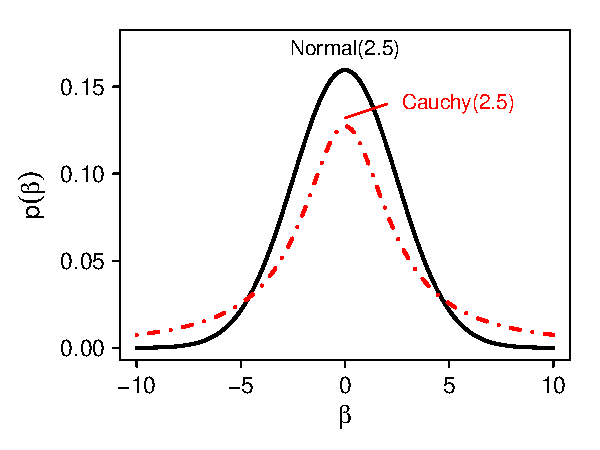
\includegraphics[scale = .8]{figs/illustrate-prior-density.pdf}
%\caption{This figure compares the Normal(2.5) and Cauchy(2.5) prior distributions. Notice that the Cauchy distribution has a similar shape to a Normal distribution, but has much heavier tails. Substantively, this prior notes that the coefficient is likely close to zero (e.g. $|\beta| < 2$), but might be quite large (e.g., $|\beta| > 5$).}\label{fig:illustrate-prior-density}
%\end{center}
%\end{figure}

As before, the posterior distribution is not easily available analytically, but one can easily use MCMC to simulate from the posterior distribution. Once a researcher has the MCMC simulations, she can obtain the point estimates and credible intervals for parameters by summarizing the simulations. 

\cite{Gelmanetal2008} design their prior distribution to be reflective of prior informative for a range of situations. In many cases, their weakly informative prior supplies too little prior information. In a few cases, it might supply too much. In any either case, it remains an open question as to whether this general prior provides a reasonable estimate of the uncertainty of the estimates for \emph{particular} research problems.

\section*{The Importance of the Prior}

While default priors, such as Zorn's suggested Jeffreys' prior or Gelman et al.'s suggested Cauchy(0, 2.5) prior are often useful as starting points, choosing a reasonable prior distribution is crucial for dealing with separation in a substantively meaningful manner. Further, whether a particular prior is reasonable depends on the particular application.

In most data analyses, the data swamp the contribution of the prior, so that the choice of prior has little effect on the posterior. However, in the case of separation, the prior essentially determines the shape of the posterior in the direction of the separation.

The likelihood has an ``S''-shape that approaches a limit as the parameter coefficient for the separating variable $s_i$ approaches infinity. Thus, for large values of the coefficient, the likelihood is essentially flat, which allows the prior distribution to drive the inferences. Thus, the prior distribution is not an arbitrary choice made for computational convenience--but an important choice that affects the inferences. We can see the importance in both theory and practice.

\subsection*{The Impact of the Prior in Theory}

Although it is intuitive that the prior drives the inferences in the direction of the separation, it is also easy to characterize the impact of the prior on a monotonic increasing likelihood in a general way. Suppose that an explanatory variable $s_i$ perfectly predicts a binary outcome variable $y_i = 1$, such that whenever $s_i = 1$, $y_i = 1$, but when $s_i = 0$, $y_i$ might equal zero or one. \cite{AlbertAnderson1984} refer to this situation as quasicomplete separation. Suppose further an additional set of covariates $X_i$ and the analyst wishes to obtain plausible estimates of coefficients the model
\begin{equation*}
Pr(y_i =1) = \text{logit}^{-1}(\beta_{cons} + \beta_s s_i +  \beta_1 x_{i1} + \beta_2 x_{i2} + ... + \beta_k x_{ik}). 
\end{equation*}
\noindent It is easy to find plausible estimates for the coefficients of $x1, x2, ..., x_k$ using the maximum likelihood, but finding plausible estimates of $\beta_{cons}$ and $\beta_{s}$ proves more difficult because maximum likelihood suggests estimates of $-\infty$ and $+\infty$, respectively. In order to obtain a plausible estimate of $\beta_{s}$ (which will, in turn, provide a plausible estimate of $\beta_{cons}$), the researcher must introduce prior information into the model. My purpose here is to characterize how this prior information impacts the posterior distribution.

In the general situation, the analyst is interested in computing and characterizing the posterior distribution of $\beta_s$ given the data. Using Bayes' Rule, the posterior distribution of $\beta = \langle \beta_{cons}, \beta_{s}, \beta_1, \beta_2, ..., \beta_k \rangle$ depends on the likelihood and the prior, so that $p(\beta | y) = p(y|\beta)p(\beta)$. In particular, the analyst might have in mind a family of priors centered at and monotonically decreasing away from zero with varying scale $\sigma$, so that $p(\beta_s) = p(\beta_s | \sigma)$, though the results below simply depend on having any proper prior distribution. Finally, suppose that the informativeness of the prior distribution depends on the scale parameter $\sigma$ that is chosen by the researcher and ``flattens'' the prior $p(\beta_s) = p(\beta_s | \sigma)$, such that as $\sigma$ increases, the rate at which the prior descends to zero decreases.

\begin{restatable}{theorem}{impact}\label{thm:impact}
For a monotonic likelihood $p(y | \beta)$ increasing in $\beta_s$, proper prior distribution $p(\beta | \sigma)$, and large $\beta_s$, the posterior distribution of $\beta_s$ is proportional to the prior distribution for $\beta_s$, so that $p(\beta_s | y) \propto p(\beta_s | \sigma)$.
\end{restatable}

\noindent \textit{Proof:} See the Technical Appendix.

Theorem \ref{thm:impact} simply implies that for large values of $\beta_s$ the posterior distribution depends almost entirely on the researcher's \emph{choice} of prior distribution. In practice, though, researchers credible intervals and measures of location to summarizes the posterior distribution.

\begin{quote}
\textsc{Practical Implication of Theorem \ref{thm:impact}:} When the direction of the separation is \emph{positive}, the prior has a small impact on the lower bound of the 90\% credible interval, a moderate impact on the measures of the location of the posterior (i.e., mean, median, and mode), and a large impact on the upper-bound of the credible interval. Similarly, when the direction of the separation is \emph{negative}, the prior has a large impact on the lower bound of the 90\% credible interval, a moderate impact on the measures of the location of the posterior (i.e., mean, median, and mode), and a small impact on the upper-bound of the credible interval.
\end{quote}

\subsection*{The Impact of the Prior in Practice}

To illustrate the impact of the prior on inferences when facing separation, I replicate a results from \cite{BarrilleauxRainey2014}, who are interesting in the effect of partisanship on governors' decisions to oppose the Medicaid expansion in their states under the Patient Protection and Affordable Care Act (ACA).\footnote{\cite{BarrilleauxRainey2014} use a logistic regression modeling the probability that a governor opposes the expansion using the following explanatory variables: the partisanship of the governor, the percent of the state's residents who are favorable toward the ACA, whether Republicans control the state legislature, the percent of the state that is uninsured, a measure of the fiscal health of the state, the Medicaid multiplier for the state, the percent of the state that is nonwhite, and the percent of the state that resides in a metropolitan area. See their paper for more details.} As the authors note, no Democratic governors opposed the expansion, which leads to a problem of separation. To see whether the choice of prior matters, I use MCMC to simulate from the posterior using Zorn's (\citeyear{Zorn2005}) and Gelman et al.'s (\citeyear{Gelmanetal2008}) suggested default prior distributions. 

Figure \ref{fig:br-coef-illustrate-importance} shows the posterior median and 90\% HPD interval for the two default priors. While the choice of prior does not affect the conclusion about the \emph{direction} of the effect, it has a large impact on the conclusion about the \emph{magnitude} of the effect. This can be especially important when researchers are making claims about the substantive importance of their estimated effects (see \citealt{Rainey2014}, \citealt{Gross2014}, and \citealt{McCaskeyRainey2014}). For example, the Cauchy(0, 2.5) prior leads to a posterior median that is over 40\% larger than the posterior median from Jeffreys' prior (4.9 compared to 3.5). The posterior mean is more than 80\% larger using the Cauchy(0, 2.5) prior (7.1 compared to 3.9). Further, both the 90\% HPD interval and the 90\% equal-tailed credible interval are more than twice as wide for the Cauchy(0, 2.5) prior. The choice between two \emph{default} priors leads to a large change in inferences.

\begin{figure}[H]
\begin{center}
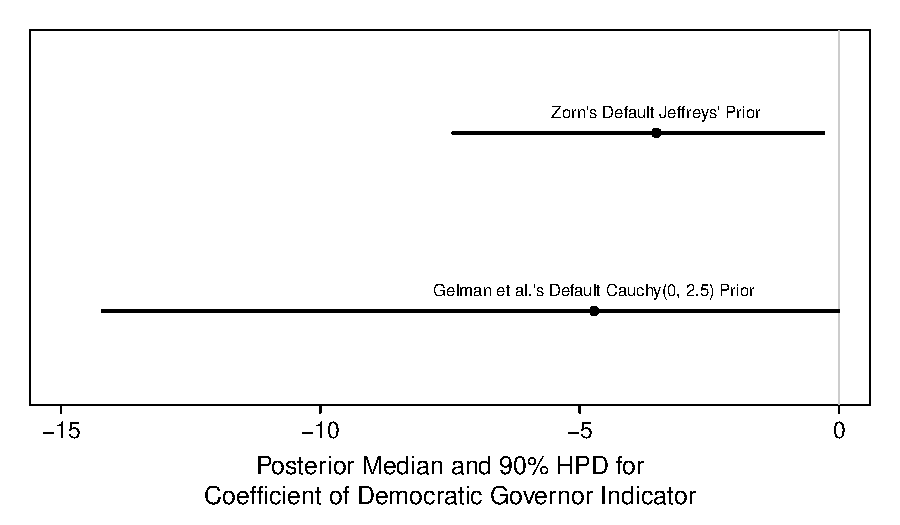
\includegraphics[scale = .8]{figs/br-coef-illustrate-importance.pdf}
\caption{This figure provides the posterior medians and 90\% HPD intervals for the coefficient of the indicator for GOP governors in the model offered by \cite{BarrilleauxRainey2014}. Notice that Jeffreys' prior, suggested by \cite{Zorn2005}, is the more informative of these priors, suggesting that a coefficient larger than about seven is quite unlikely. On the other hand, the credible interval using the Cauchy(0, 2.5) prior, as suggested by \cite{Gelmanetal2008}, is about \emph{twice} as wide as the credible interval from Jeffreys' prior, suggesting that effects as large as about 15 are plausible. Further, the posterior median from the Cauchy(0, 2.5) prior is about 40\% larger than the posterior median from Jeffreys' prior.}\label{fig:br-coef-illustrate-importance}
\end{center}
\end{figure}

Figure \ref{fig:bf-posterior-density-illustrate-importance} shows the posterior distribution for the coefficient for the indicator of Republican governors. Notice that these two \emph{default} priors lead to different posterior distributions. Notice, in particular, that the choice of the prior has a large impact on the right-hand side of the posterior, as suggested by Theorem \ref{thm:impact}. The more informative Jeffreys' prior leads to a more peaked posterior distribution that rules out coefficients larger than about seven. The less informative Cauchy(0, 2.5) prior leads to the conclusion that much larger effects, such as 15 are plausible. These differences are not trivial--there are large differences in the posterior distributions, and these differences can affect the conclusions that the researchers draw about the likely magnitude of the effect.

\begin{figure}[H]
\begin{center}
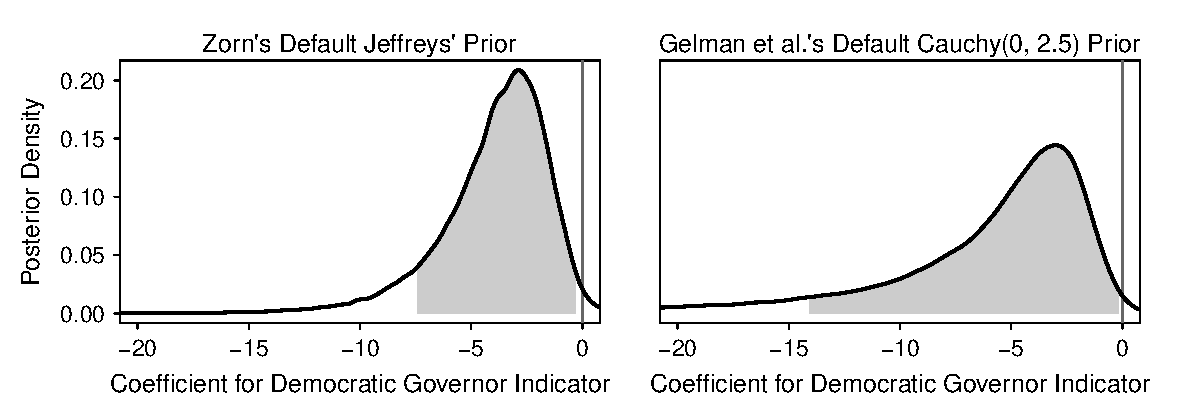
\includegraphics[scale = .8]{figs/br-posterior-density-illustrate-importance.pdf}
\caption{This figure shows the posterior distribution for the coefficient of the indicator for GOP governors in the model offered by \cite{BarrilleauxRainey2014} for different default prior distributions. The grey shading indicates the 90\% HPD interval. Notice that the location and the spread of the posterior depend on the prior chosen, especially the right-hand side of the distribution, as suggested by Theorem \ref{thm:impact}}\label{fig:bf-posterior-density-illustrate-importance}
\end{center}
\end{figure}

%Figure \ref{fig:br-coef-illustrate-importance} shows how the choice of prior impacts the 90\% credible interval. Notice that different prior distributions lead to different conclusions about the plausible values of the effect. In particular, different priors lead to different conclusions about the upper-bound on the plausible effect sizes. For example, Jeffreys' prior, the default proposed by \cite{Zorn2005} and \cite{HeinzeSchemper2002}, suggests the effect lies in the range $\beta_{\text{GOP Gov.}} \in [0.9, 8.4]$, with a posterior mean of 3.9. On the other hand, the less informative Cauchy(2.5) prior, the default proposed by \cite{Gelmanetal2008}, suggests the effect lies in the range $\beta_{\text{GOP Gov.}} \in [1.0, 22.5]$, with a posterior mean of 7.3. A simple change from one proposed default to another more than doubles the upper bound on the 90\% credible interval and almost doubles the posterior mean. Further, the Cauchy(5) prior, a plausible prior if one believes the effect might be large, produces the upper-bound on the 90\% credible interval from is more than four times larger than the upper-bound produced by Jeffrey's prior. The posterior mean from the Cauchy(5) prior is larger falls above the upper-bound from the 90\% credible interval from Jeffrey's prior.

%
%This leads us to conclude that the choice of prior matters--it affects the inferences that we draw from the data. It is not sufficient to rely on the prior distribution designed as a default for other purposes. Instead, we must rely on prior distributions that represent actual prior information about the likely magnitude of the coefficients.


\section*{Choosing an Informative Prior}

While is often sufficient to rely on default priors, this is not the case if one is interested in obtaining reasonable measures of uncertainty under separation. Indeed, in the replication of \cite{BarrilleauxRainey2014} above, I show that the overall posterior distribution, the width of the 90\% credible interval, and the posterior median largely depend on the prior one chooses . This implies that researchers relying on default priors alone risk under- or over-representing their confidence in the magnitude of the effect.

When facing separation, our goal is to choose a prior distribution that satisfies three properties:
\begin{enumerate}
\item \emph{Pools toward zero.} While the ultimate goal is to choose a prior distribution based on actual prior information, the prior distribution should also be appropriately conservative. As mentioned before, the prior distribution largely drives the inferences in the direction of the separation. In this case, a non-central prior distribution in the direction of the separation has an especially large impact on the inferences. For this reason, I focus on prior distributions centered at zero to conservatively pool coefficients downward toward zero \citep{GelmanJakulin2007}.
\item Allow plausible effects. The prior distribution should assign realistic prior probabilities to estimates that are \textit{a priori} plausible. 
\item Rule out implausible effects. The prior distribution should assigned essentially know prior probability to estimates that are \textit{a priori} implausible.
\end{enumerate}

To assess the reasonableness of the prior distribution, the research might examine the prior predictive distribution and ask herself whether the prior and model produce a distribution for the data that matches her prior beliefs. Under the Bayesian framework, the researcher has a fully specified model $p(y_{new}|\theta)p(\theta)$ and can thus simulate hypothetical data $y_{new}$ from the model prior to observing the data. The distribution of the unobserved outcome $y_{new}$ is given by $p(y_{new}) = \int p(y_{new} | \theta)p(\theta) d\theta$ \citep{Box1980}. In practice, this process involves Clarify-like simulation \citep{KingTomzWittenberg2000}, but rather than using the asymptotic posterior (e.g., $\beta_{sim} \sim N\left[\hat{\beta}^{mle}, I(\hat{\beta}^{mle})^{-1}\right]$), researchers simulate the model parameters from the prior distribution. Just as a researcher can use simulation to interpret the coefficient estimates of nonlinear models, she can use simulation to interpret the prior distribution.

\begin{defn}[Prior Predictive Distribution] The prior predictive distribution (PPD), denoted as $p(y_{new})$, is the prior distribution of hypothetical data, so that $p(y_{new}) = \int\limits_{-\infty}^{\infty} p(y | \beta)p(\beta)d(\beta)$.
\end{defn}

However, it is difficult to work with more than one dimension of the prior distribution. Specifying the full prior distribution requires simultaneously choosing prior distributions for the $k + 1$ explanatory variables, as well as the relationships among these variables (e.g., family, location, scale, and correlations of all the parameters). But only specific $k + 1$ dimensional distribution is practically importance when addressing separation. In particular, the researcher can simplify the focusing in two specific ways.
\begin{enumerate}
\item \emph{Focus only on the separated coefficient.} Since the data swamp the prior for all but the separated coefficient, the only relevant ``slices'' of the prior distribution are those in which all other coefficients are near their maximum likelihood estimates.
\item \emph{Focus in the direction of the separation.} The likelihood also swamps the prior in the direction opposite the separation. Unless the researcher has an extremely small data set (i.e., smaller than \cite{BarrilleauxRainey2014}, who have $N = 50$), the the likelihood essential rules out values less [greater] than zero when the direction of separation is positive [negative].
\end{enumerate}

I refer to this simplified focus as the \emph{partial} prior predictive distribution.

\begin{defn}[Partial Prior Predictive Distribution]\label{def:pppd} The \underline{partial} prior predictive distribution (P$^3$D), denoted as $p^*(y_{new})$, is the prior distribution of $y_{new}$ given that the separated coefficient lies in the direction of the separation and all other coefficients equal their maximum likelihood estimates, so that $p^*(y_{new}) = \int_{0}^{\infty} p(y | \beta_s, \hat{\beta}_{-s}^{mle})p(\beta_s | \beta_s \geq 0)d(\beta_s)$ when $\hat{\beta}_{s}^{mle} = +\infty$ and $p^*(y_{new}) = \int_{-\infty}^{0} p(y | \beta_s, \hat{\beta}_{-s}^{mle})p(\beta_s | \beta_s \leq 0)d(\beta_s)$ when $\hat{\beta}_{s}^{mle} = -\infty$.
\end{defn}

For example, in \cite{BarrilleauxRainey2014}, we do not need to use prior information to obtain reasonable estimates for our measures of need and public opinion. Further, because no Democratic governors opposed the Medicaid expansion, then we do not need the prior to rule out large \textit{positive} effects for Democratic partisanship. In both cases, the likelihood is sufficiently informative. 

However, we do need to use the prior to rule out large \textit{negative} effects, since the likelihood cannot effectively rule out implausibly large negative effects. The likelihood is monotonically decreasing in the coefficient for the indicator of Democratic governors. The larger the negative effect, the more likelihood separation would occur. The usual maximum likelihood, therefore, provides implausibly large estimates and unreasonable standard errors. Theorem \ref{thm:impact} provides a more formal treatment of this intuition, but prior information is essential to obtain reasonable estimates and measures of uncertainty. 

Choosing a prior, though, requires some effort. As I show above, default priors can lead to much different conclusions so it is essential to build actual prior information into the model. In order to choose a reasonable, informative prior distribution, researchers need to obtain the partial prior predictive distribution defined in Definition \ref{def:pppd}. The following steps describe how researchers can simulate from the partial prior predictive distribution and use the simulations to check the reasonableness of the choice.
\begin{enumerate}
\item Estimate the model coefficient using maximum likelihood, giving the coefficient vector $\hat{\beta}^{mle}$. Include the separating variable $s_i$ in the model. Of course, this leads to implausible estimates for $\beta_s$, but the goal purpose is to choose reasonable values at which to fix the \emph{other} parameters in order to focus on a single slice of the full prior. 
\item Choose a prior distribution $p(\beta_s)$ for the separating variable $s$ that is centered at zero. The most common choice is the scaled $t$ distribution, which has the normal and Cauchy families as special cases ($df = \infty$ and $df = 1$, respectively). 
\item Choose a large number of simulations $n_{sims}$ to perform (e.g., $n_{sims} \geq 10,000$) and for $i$ in 1 to $n_{sims}$ (e.g., $n_{sims} \geq 10,000$), do the following:
	\begin{enumerate}
	\item Simulate $\tilde{\beta}^{[i]}_s \sim p(\beta_s)$ and keep only those simulations in the direction of the separation (e.g., $\tilde{\beta}_s \geq 0$ when $\hat{\beta}_{s}^{mle} = +\infty$ and $\tilde{\beta}_s \leq 0$ when $\hat{\beta}_{s}^{mle} = -\infty$)
	\item Replace $\hat{\beta}_s^{mle}$ in $\hat{\beta}^{mle}$ with $\tilde{\beta}^{[i]}_s$, yielding the vector $\tilde{\beta}^{[i]}$.
	\item Calculate the store the quantity of interest $\tilde{q}^{[i]} = q\left(\tilde{\beta}^{[i]}\right)$. This quantity of interest might be a first-difference or risk-ratio, for example.
	\end{enumerate}
\item Summarize the simulations $\tilde{q}$ using quantiles, histograms, or density plots. If the prior is inadequate, then update the prior distribution $p(\beta_s)$.
\end{enumerate}

Given that the inference can be highly dependent on the choice of prior, I recommend that the researcher choose at least three prior distributions: (1) an \emph{informative} prior distribution that represents her actual beliefs, (2) a highly \emph{skeptical} prior distribution that suggests the effect is likely small, and (3) a highly \emph{optimistic} prior that represents the suggests the effect might be very large. Combined with Zorn's (\citeyear{Zorn2005}) and Gelman et al.'s (\citeyear{Gelmanetal2008}) suggested defaults, these provide range of prior distributions that researchers can use to evaluate their inferences.

\section*{Estimating the Full Model}

Once the researcher obtains a reasonable prior distribution as well as several to use for robustness checks, she must use MCMC to obtain simulations from the posterior. \citeyear{Zorn2005} and \cite{Gelmanetal2008} suggest variations on maximum likelihood to quickly obtain estimates and confidence intervals, but normal approximation used to simulate the estimates and calculate quantities of interest \citep{KingTomzWittenberg2000} is particularly inaccurate under separation. As an alternative, I recommend the researcher use MCMC to simulation directly from the posterior distribution. The researcher can then use these simulations to calculate point estimates and confidence intervals for any desired quantity of interest. For the informative $p_{\text{inf}}(\beta_s)$, skeptical $p_{\text{skep}}(\beta_s)$, and enthusiastic $p_{\text{opt}}(\beta_s)$ priors , I suggest the model:

\begin{equation*}
Pr(y_i =1) = \text{logit}^{-1}(\beta_{cons} + \beta_s s_i +  \beta_1 x_{i1} + \beta_2 x_{i2} + ... + \beta_k x_{ik})
\end{equation*}
\begin{equation*}
\beta_s \sim  p_k(\beta_s) \text{, for } k \in \{\text{inf, skep, enth}\},
\end{equation*}
with improper, constant priors on the other model coefficients.

\section*{Application: Nuclear Proliferation and War}

A recent debate emerged in the conflict literature between \cite{Rauchhaus2009} and \cite{BellMiller2014} that revolves around the issue of separation. \cite{Rauchhaus2009} hypothesizes that ``[t]he probability of major war between two states will decrease if both states possess nuclear weapons (p. 262).'' Summarizing his empirical results, Rauchhaus writes:

\begin{quote} 
The hypotheses on nuclear symmetry find strong empirical support. The probability of a major war between two states is found to decrease when both states possess nuclear weapons (p. 269).
\end{quote}

Despite using the same data, \cite{BellMiller2014} claim that ``nonnuclear dyads are in fact no more likely to fight wars than nonnuclear dyads (p. 9).'' Their disagreement hinges, in part, on whether and how to handle separation, because no nuclear dyad in Rauchhaus data engage in war.\footnote{\cite{BellMiller2014} also disagree with a coding decision of \cite{Rauchhaus2009}, but that portion of their argument is less relevant to my purpose. Instead, my goal is to illustrate how one might choose a reasonable prior distribution and highlight the importance of the choice of prior.} \cite{Rauchhaus2009} ignores the separation and estimate that nonnuclear dyads are about 2.7 million times more likely to go to war than symmetric nuclear dyads. \cite{BellMiller2014}, on the other hand, use Jeffreys' (\citeyear{Jeffreys1946}) invariant prior, as suggested by \cite{Zorn2005}, and estimate that nonnuclear dyads are only about 1.6 times more likely to engage in war. Because these authors use very different prior distributions, they reach very different conclusions. This raises important questions. First, if we build a reasonable, informative prior distribution, does it support Rauchhaus' position of a meaningful effect or Bell and Miller's position of essentially no effect? Second, how robust is the conclusion to a range of more and less informative prior distributions?

\subsection*{Prior}

The first step in dealing with the separation in a principled manner is to choose a prior distribution that represents actual prior information. To choose a reasonable prior, I follow the process above to generate a partial prior predictive distribution for the risk-ratio that \cite{BellMiller2014} emphasize. I experimented with a range of prior distributions, from a varieties of families, but settled on the normal family. After some experimentation, I selected a normal distribution with mean zero and standard deviation 4.5 to serve as an informative prior and represent my own prior beliefs. 

To evaluate the robustness of any statistical claims to the choice of prior, I also selected a highly skeptical and highly enthusiastic prior. I also selected a normal distribution with mean zero and standard deviation two to serve as a skeptical prior that represents the belief that any pacifying effect of nuclear weapons is small. Finally, I selected a normal distribution with mean zero and standard deviation eight to serve as a skeptical prior that represents the belief that the pacifying effects of nuclear weapons might be quite large. Because the likelihood is highly informative about the other parameters in the model, I place an improper, flat prior for these parameters. Figure \ref{fig:bm-pppd-hist} shows the partial prior predictive distributions for the informative, skeptical, and enthusiastic prior distributions. For convenience, Table \ref{tab:bm-pppd-deciles} provides the deciles of the PPPDs shown in Figure \ref{fig:bm-pppd-hist}. 

\begin{figure}[H]
\begin{center}
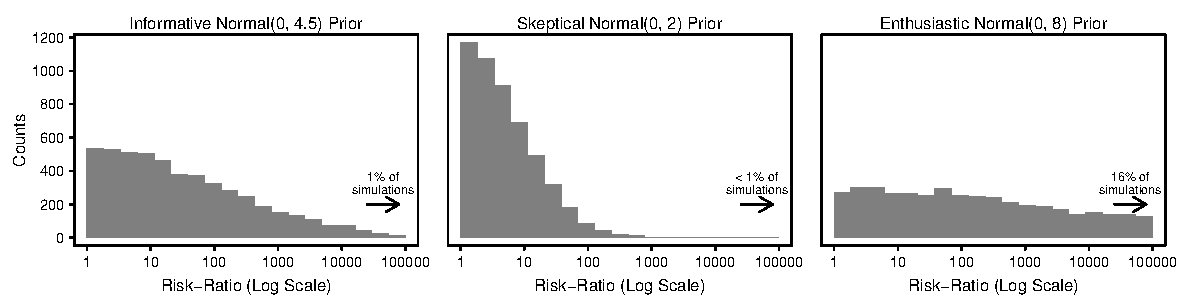
\includegraphics[scale = .8]{figs/bm-pppd-hist.pdf}
\caption{This figure shows the partial prior predictive distribution for the risk-ratio of war in nonnuclear to nuclear dyads. The risk-ratio is tells us how many times more likely war is in non-nuclear dyads compared to nuclear dyads. Notice that the informative prior treats effects smaller than 100 as plausible, but essentially rules out effects larger than 10,000. Gelman's suggested default places more weight closer to zero and more weight above 10,000. The skeptical prior essentially rules out effects larger than 100, while the enthusiastic prior treats effects between 1 and 100,000 as essentially equally likely.}\label{fig:bm-pppd-hist}
\end{center}
\end{figure}

% latex table generated in R 3.1.1 by xtable 1.7-3 package
% Sun Oct  5 07:07:18 2014
\begin{table}[H]
\centering
{\scriptsize
\begin{tabular}{|cccccccccc|}
  \hline
 & 10\% & 20\% & 30\% & 40\% & 50\% & 60\% & 70\% & 80\% & 90\% \\ 
  \hline
Informative Normal(0, 4.5) Prior &       1.7 &       3.1 &       5.6 &      10.3 &      19.5 &      44.1 &      98.8 &     296.9 &   1,577.7 \\ 
  Skeptical Normal(0, 2) Prior &       1.3 &       1.7 &       2.2 &       2.9 &       3.9 &       5.4 &       8.3 &      13.2 &      26.7 \\ 
  Enthusiastic Normal(0, 8) Prior &       2.9 &       8.1 &      24.7 &      76.5 &       256 &     987.6 &   5,300.9 &  42,466.7 & 643,954.6 \\ 
   \hline
\end{tabular}
}
\caption{This table provides the deciles prior predictive distribution for the 
                  risk-ratio of war in nonnuclear and nuclear dyads. The risk-ratio is 
                  tells us how many times more likely war is in non-nuclear dyads compared 
                  to nuclear dyads. Notice that that the, informative prior suggests a median 
                  risk-ratio of about 20, which is a large, but plausible effect. The skeptical prior suggests a median 
                  ratio of about 4 and the enthusiastic prior suggests a median ratio of over 
                  200.} 
\label{tab:bm-pppd-deciles}
\end{table}


Notice that the skeptical prior suggests that risk-ratios above and below 4 are equally likely (i.e., 50th percentile of the PPPD is 3.9), while the enthusiastic prior suggests that effects above and below 220 are equally likely. The informative prior, on the other hand, suggests (more reasonably, in my view) that the effect is equally likely to fall above and below 20. These three prior distributions, along with the defaults suggested by \cite{Zorn2005} and \cite{Gelmanetal2008}, provide a range of distributions to represent a range of prior beliefs.

\subsection*{Posterior}

Figure \ref{fig:bm-posterior-density} shows the posterior distributions for the coefficient of the indictor of nuclear dyads from the informative, skeptical, enthusiastic, and two default prior distributions. The areas shaded grey indicate the 90\% credible intervals (a highest posterior density, or HDP, interval, akin to a 90\% confidence interval).\footnote{Obviously, we could define many intervals that have 90\% chance of containing the true parameter. However, the HPD interval is theoretically appealing because it is the \emph{shortest} of these intervals. See \citet[esp. pp. 48-51]{Gill2008} and \citet[esp. p. 448]{CasellaBerger2002}.} Notice that the location (e.g., peak or mode), shape, scale, and credible interval depend on the choice of prior. While the magnitude of this coefficient is not easily interpretable, notice that the Gelman et al.'s Zorn's (\citeyear{Gelmanetal2008}) suggested default prior is somewhat similar to the informative prior, but Zorn's (\citeyear{Zorn2005}) suggested default is quite similar to the \emph{skeptical} prior. Thus, these distributions illustrate that the prior is important when dealing with separation. Instead, it is a critical step in obtaining reasonable inferences.

\begin{figure}[H]
\begin{center}
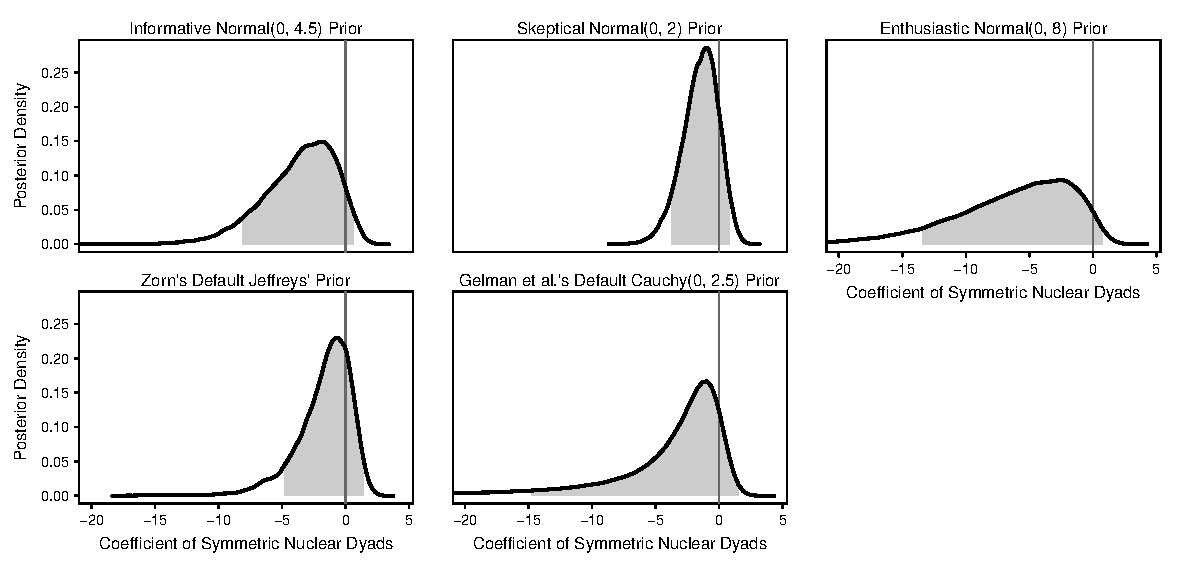
\includegraphics[scale = .8]{figs/bm-posterior-density.pdf}
\caption{This figure shows the posterior distribution for the logit coefficient using each of the five prior distributions.  The grey shading indicates the 90\% highest posterior density (HPD) . Notice that the choice of prior has a large effect on the inferences. For example, the enthusiastic prior suggests the ratio might be as large as -13, while the skeptical prior suggests the ratio might be as large as -4. Importantly, notice the similarity between the posterior from Zorn's (\citeyear{Zorn2005}) suggested default and the skeptical prior, in terms of their peak (i.e., mode), shape, and highest posterior density.}\label{fig:bm-posterior-density}
\end{center}
\end{figure}

I now turn to the posterior distribution of the risk-ratios--the key quantity of interest in the debate between \cite{BellMiller2014} and \cite{Rauchhaus2009}. Figure \ref{fig:bm-rr} presents the posterior medians and the 90\% HPD intervals for each prior. While an initial glance at the figure shows substantial variation in the point estimates and the width of the intervals, notice that these are plotted on the log scale (otherwise the wider intervals dominate the plot). Notice that the informative prior suggests the true risk-ratio has about a 90\% chance of falling between about 0.1 and about 2000, with a posterior median of about 25.\footnote{It is worth pointing out that these wide confidence interval suggest that, although the HPD intervals overlap zero, these data do not warrant a conclusion of ``no effect'' (see \citealt{Rainey2014}).} The skeptical prior, on the other hand, suggests the risk-ratio has about a 90\% chance of falling between 0.1 and 30, with a posterior median of about 4. The enthusiastic prior suggests the risk-ratio has about a 90\% chance of falling between 0.1 and 500,000. The inferences from these priors are \emph{very} different. 

Further, the 90\% credible interval using Zorn's (\citeyear{Zorn2005}) default is \emph{much} narrower than the informative prior, and the posterior median of Zorn's suggested default prior is even smaller than the \emph{skeptical} prior. For this particular application, Gelman's suggested default more closely matches the informative prior, though notice that the point estimate is less than half and the upper-bound of the credible interval is ten times larger than than the point estimate and upper-bound of the credible interval from the informative prior.

%\begin{figure}[H]
%\begin{center}
%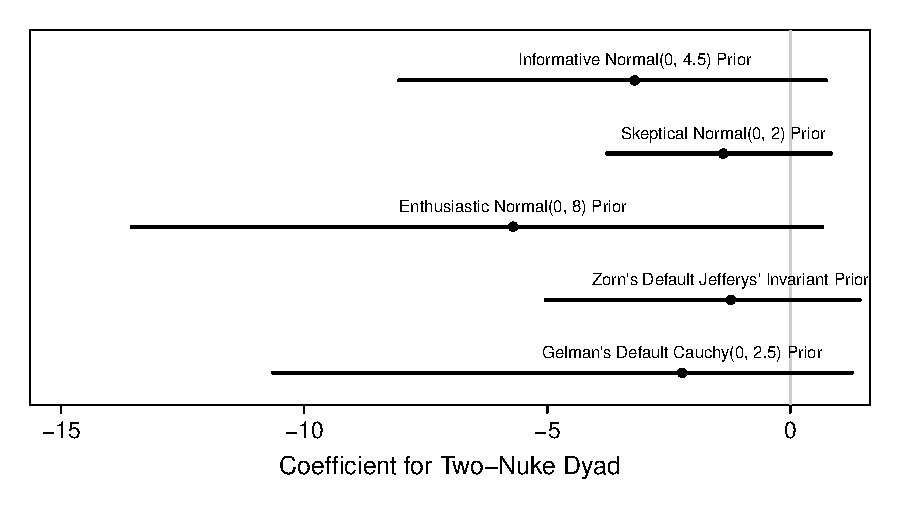
\includegraphics[scale = .8]{figs/bm-coef.pdf}
%\caption{}\label{fig:bm-coef}
%\end{center}
%\end{figure}

\begin{figure}[H]
\begin{center}
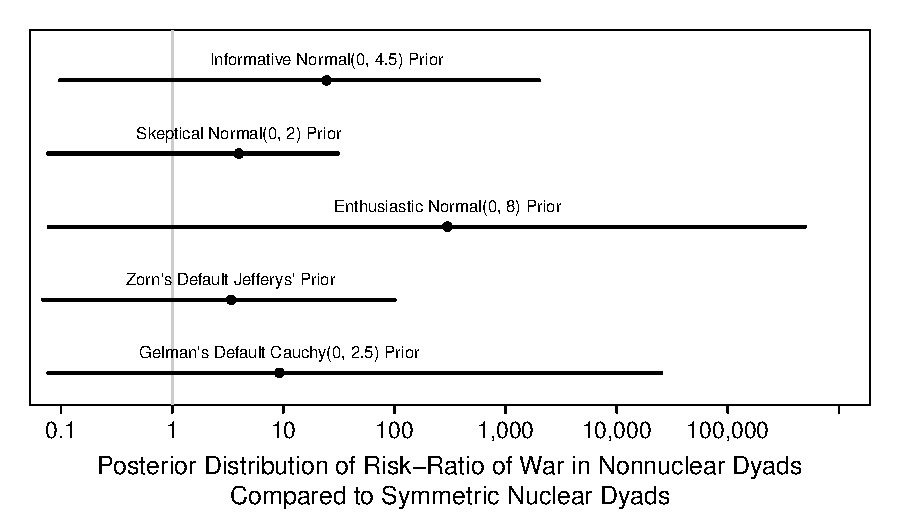
\includegraphics[scale = .8]{figs/bm-rr.pdf}
\caption{This figure shows the posterior median and 90\% highest posterior density (HPD) for the risk-ratio using each of the five prior distributions \emph{on the log scale}. Notice that the choice of prior has a huge effect on the inferences about the risk-ratio. For example, the skeptical prior suggests the ratio might be as large as 31, while the enthusiastic prior suggests the ratio might be as large as 500,000. Also, notice that the posterior median from Zorn's proposed default prior is \emph{smaller} than the posterior median from the skeptical prior.}\label{fig:bm-rr}
\end{center}
\end{figure}

%% latex table generated in R 3.1.1 by xtable 1.7-3 package
% Mon Oct  6 05:01:40 2014
\begin{table}[H]
\centering
{\scriptsize
\begin{tabular}{|cccc|}
  \hline
 & Lower-Bound of 90\% HPD & Posterior Median & Upper-Bound of 90\% HPD \\ 
  \hline
Informative Normal(0, 4.5) Prior &       0.1 &      24.5 &   1,986.4 \\ 
  Skeptical Normal(0, 2) Prior &       0.1 &         4 &      31.2 \\ 
  Enthusiastic Normal(0, 8) Prior &       0.1 &     299.2 & 499,043.2 \\ 
  Zorn's Default Jeffreys' Prior &       0.1 &       3.4 &     100.2 \\ 
  Gelman et al.'s Default Cauchy(0, 2.5) Prior &       0.1 &       9.2 &  25,277.4 \\ 
   \hline
\end{tabular}
}
\caption{This table provides lower- and upper-bounds for the 90% HPD and posterior medians 
              for the five prior distributions I consider.} 
\label{tab:bm-pppd-deciles}
\end{table}


Finally, I use the posterior distributions from each prior to calculate the probability that the presence of nuclear weapons make war less likely (i.e., the probability that the risk-ratios shown in Figure \ref{fig:bm-rr} are greater than one). Recall Rauchhaus' hypothesis that nuclear weapons decrease the chance of war. These probabilities can be thought of as the probability that Rauchhaus' hypothesis is correct. Following the standard of $p \leq 0.05$ as offering strong evidence against the null hypothesis, it is reasonable to take $Pr(RR > 1) \geq 0.95$ as strong evidence for the research hypothesis. Figure \ref{fig:bm-pr-hypothesis} shows the probability that the hypothesis is correct for each prior distribution. Notice that while only the enthusiastic prior falls above the 0.95 standard, the evidence for the claim is at least suggestive. Perhaps most importantly for my purposes, Zorn's suggested default leads to the \emph{least} evidence in favor of Rauchhaus' hypothesis--even the skeptical prior provides more evidence for Rauchhaus' claim.

\begin{figure}[H]
\begin{center}
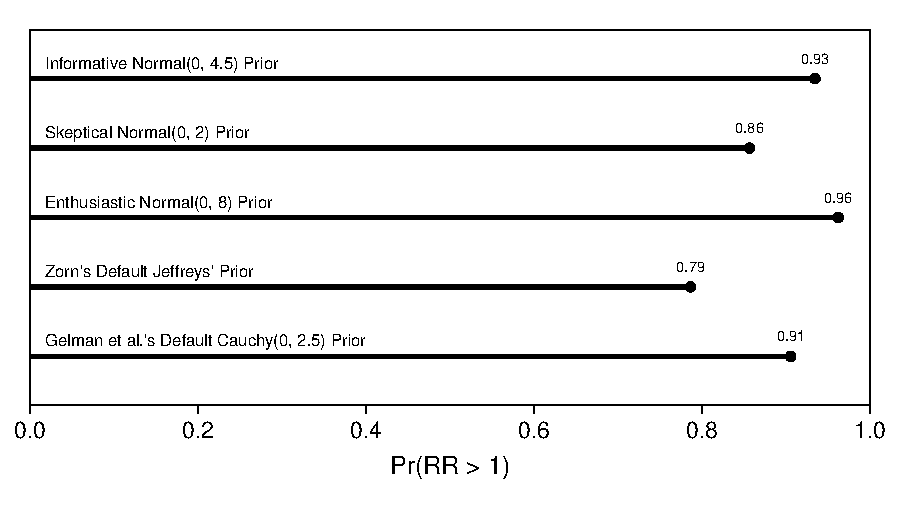
\includegraphics[scale = .8]{figs/bm-pr-hypothesis.pdf}
\caption{This figure shows the posterior probability of the hypothesis that nonnuclear dyads are \emph{more} likely to engage in war than symmetric nuclear dyads for each of the five prior distribution. From a hypothesis testing perspective, the evidence for the hypothesis is borderline or suggestive for each prior. However, notice that the skeptical prior, perhaps held by a skeptical researcher who believes the pacifying effect of nuclear weapons is small or nil, yields \emph{greater} evidence for the hypothesis than Jeffreys' invariant prior suggested as a default by \cite{Zorn2005}.}\label{fig:bm-pr-hypothesis}
\end{center}
\end{figure}

\subsection*{Conclusion}

Separation is a relatively common situation in political science. It is also an unusual ``problem'' in political science because the effects in the sample are ``too big'' for maximum likelihood. In this situation, dropping the separating variables (i.e., deliberate specification bias) and interpreting the implausible coefficients and standard errors are particularly unattractive options. But even the most principled solution to date, the incorporation of prior information via default priors (\citealt{Zorn2005}, \citealt{Gelmanetal2008}), have shortcomings.

First, the normal approximations necessary to simulate from these default prior distributions perform poorly. While it is possible to use profile likelihood methods to obtain more accurate confidence intervals for the coefficients (\citealt{Zorn2005}, \cite{HeinzeSchemper2002}, \cite{McCullaghNelder1989}), it is difficult to translate these intervals into confidence intervals for quantities of interest. I provide the computational tools to simulate directly from the posterior using both Zorn's (\citeyear{Zorn2005}) and Gelman et al.'s Zorn's (\citeyear{Gelmanetal2008}) suggested default priors.

Second, the application illustrates what Theorem \ref{thm:impact} proves--under separation, the choice of prior affects substantive conclusions. Even the predominant default priors used to deal with separation can provide very different inferences. A carefully-chosen, informative prior is an essential part of obtaining reasonable inferences under separation. What does this mean for applied researchers? I suggest two implications:
\begin{enumerate}
\item When facing separation, the choice of prior matters. Researchers must carefully choose a prior that represents actual prior information, otherwise, the point and interval estimates will be too large.
\item In addition to carefully choosing an informative prior that represents her own beliefs, the researcher should show how the inferences change for a range of prior distributions. In the debate between \cite{BellMiller2014} and \cite{Rauchhaus2009}, the choice of prior almost completely drives the inferences about the likely magnitude of the risk-ratio. Thus, to the extent that there is disagreement about the prior, there will be disagreement about the results. In particular, I suggest that researchers report the key quantities of interest for a highly skeptical prior, an enthusiastic prior, and the two default priors suggested by \cite{Zorn2005} and \cite{Gelmanetal2008}.
\end{enumerate}

When facing separation, researchers must \emph{carefully} choose a prior distribution to rule out implausibly large effects. This paper introduces the concept of a partial prior predictive distribution and the associated computational tools to help researchers choose a prior distribution that represents actual prior information for their particular research problem. By presenting results from a range of prior distributions, including an informative prior, researchers can increases the transparency, credibility, and accuracy of their inferences when dealing with separation.

\clearpage
\bibliographystyle{apsr_fs}
\bibliography{/Users/carlislerainey/Dropbox/papers/bibliography/bibliography.bib}

\clearpage
\begin{appendix}
\begin{center}
\LARGE{\textbf{Technical Appendix}}\vspace{4mm}
\end{center}

\section*{Proof of Theorem \ref{thm:impact}}

Recall Theorem \ref{thm:impact}:

\impact*

\begin{proof}
Due to separation, $p(y|\beta)$ is monotonic increasing in $\beta_s$ to a limit $\underline{\mathscr{L}}$, so that $\displaystyle \lim_{\beta_s \to \infty} p(y | \beta) = \underline{\mathscr{L}}$. By Bayes' rule, 
\begin{equation*}
p(\beta | y) = \dfrac{p(y | \beta)p(\beta | \sigma)}{\int\limits_{-\infty}^{\infty}p(y | \beta)p(\beta | \sigma)d\beta} = \dfrac{p(y | \beta)p(\beta | \sigma)}{\underbrace{p(y | \sigma)}_{\text{constant w.r.t. }\beta}}. 
\end{equation*}
Integrating out the other parameters $\beta_{-s} = \langle \beta_{cons}, \beta_1, \beta_2, ..., \beta_k \rangle$ to obtain the posterior distribution of $\beta_s$, 
\begin{equation}\label{eqn:int-post}
p(\beta_s | y) = \dfrac{\int\limits_{-\infty}^{\infty}p(y | \beta)p(\beta | \sigma)d\beta_{-s}}{p(y | \sigma)}, 
\end{equation}
and the prior distribution of $\beta_s$, 
\begin{equation*}
p(\beta_s | \sigma) = \int\limits_{-\infty}^{\infty}p(\beta | \sigma)d\beta_{-s}.
\end{equation*}
Notice that $p(\beta_s | y) \propto p(\beta_s | \sigma)$ iff $\dfrac{p(\beta_s | y)}{p(\beta_s | \sigma)} = k$, where the constant $k \neq 0$.Thus, Theorem \ref{thm:impact} implies that
\begin{equation*}
\lim _{\beta_s \to \infty} \dfrac{p(\beta_s | y)}{p(\beta_s | \sigma)} = k
\end{equation*}
Substituting in Equation \ref{eqn:int-post},
\begin{equation*}
\lim _{\beta_s \to \infty} \dfrac{\frac{\int\limits_{-\infty}^{\infty}p(y | \beta)p(\beta | \sigma)d\beta_{-s}}{p(y | \sigma)}}{p(\beta_s | \sigma)} = k.
\end{equation*}
Multiplying both sides by $p(y | \sigma)$, which is constant with respect to $\beta$, 
\begin{equation*}
\lim _{\beta_s \to \infty} \dfrac{\int\limits_{-\infty}^{\infty}p(y | \beta)p(\beta | \sigma)d\beta_{-s}}{p(\beta_s | \sigma)} = kp(y | \sigma).
\end{equation*}
Setting $\int\limits_{-\infty}^{\infty}p(y | \beta)p(\beta | \sigma)d\beta_{-s} = p(y | \beta_s) p(\beta_s | \sigma)$, 
\begin{equation*}
\lim _{\beta_s \to \infty} \dfrac{p(y | \beta_s) p(\beta_s | \sigma)}{ p(\beta_s | \sigma)} = kp(y | \sigma).
\end{equation*}
Canceling $p(\beta_s | \sigma)$ in the numerator and denominator,
\begin{equation*}
\lim _{\beta_s \to \infty} p(y | \beta_s) = kp(y | \sigma).
\end{equation*}
Recalling that $\displaystyle \lim_{\beta_s \to \infty} p(y | \beta) = \underline{\mathscr{L}}$ and substituting,
\begin{equation*}
\underline{\mathscr{L}}= kp(y | \sigma),
\end{equation*}
which implies that $k = \dfrac{p(y | \sigma)}{\underline{\mathscr{L}}}$, which is a positive constant.
\end{proof}

\end{appendix}
\end{document}



